\section{Overview of Results}
\begin{comment}
    This covers an area different from the 'Testing'
chapter, and relates to the understanding and analysis
of the algorithm, program, or hardware behaviour.
Where the deliverable is a product with easily
quantified performance then the previous Chapter
shows how functional correctness is established,
while this Chapter shows qualitatively or
quantitatively how well the product works. The list
below shows typical content, not all of this will be
applicable to all projects.

\begin{itemize}
    \item An empirical relationship between
    parameters and results may be investigated,
    typically through the use of appropriate
    graphs.
    \item Where theory predicts aspects of
    performance the results can be compared
    with expectation and differences noted and (if
    possible) explained.
    \item Semi-empirical models of behaviour may be
    developed, justified, and tested.
    \item The types of experiments/simulations that
    were carried out should be described. Why
    were certain experiments carried out but not
    others? What were the important parameters
    in the simulation and how did they affect the
    results? If there are very many graphs and
    tables associated with this chapter they may
    be put in the Appendix, but it is generally
    better to keep these close to the text they
    illustrate, as this is easier for the reader.
\end{itemize}
\end{comment}

\textcolor{red}{For all results:}

\textcolor{red}{1. Ensure all results have units (if it doesn't have units, it's A.U for arbitrary units)}

\textcolor{red}{2. If you have sub figures or diagram, label them a, b, c and include a short description in the caption.}


\subsection{Overview of testing parameters}

\begin{itemize}
    \item KEEP ADDING MORE STUFF
    \item GPU used
    \item Features used for each set of results
    \item Learning rate
    \item Optimizer
    \item Loss function
    \item 
\end{itemize}

\subsection{Performance of AlexNet architecture}

\begin{figure}[H]
    \centering
    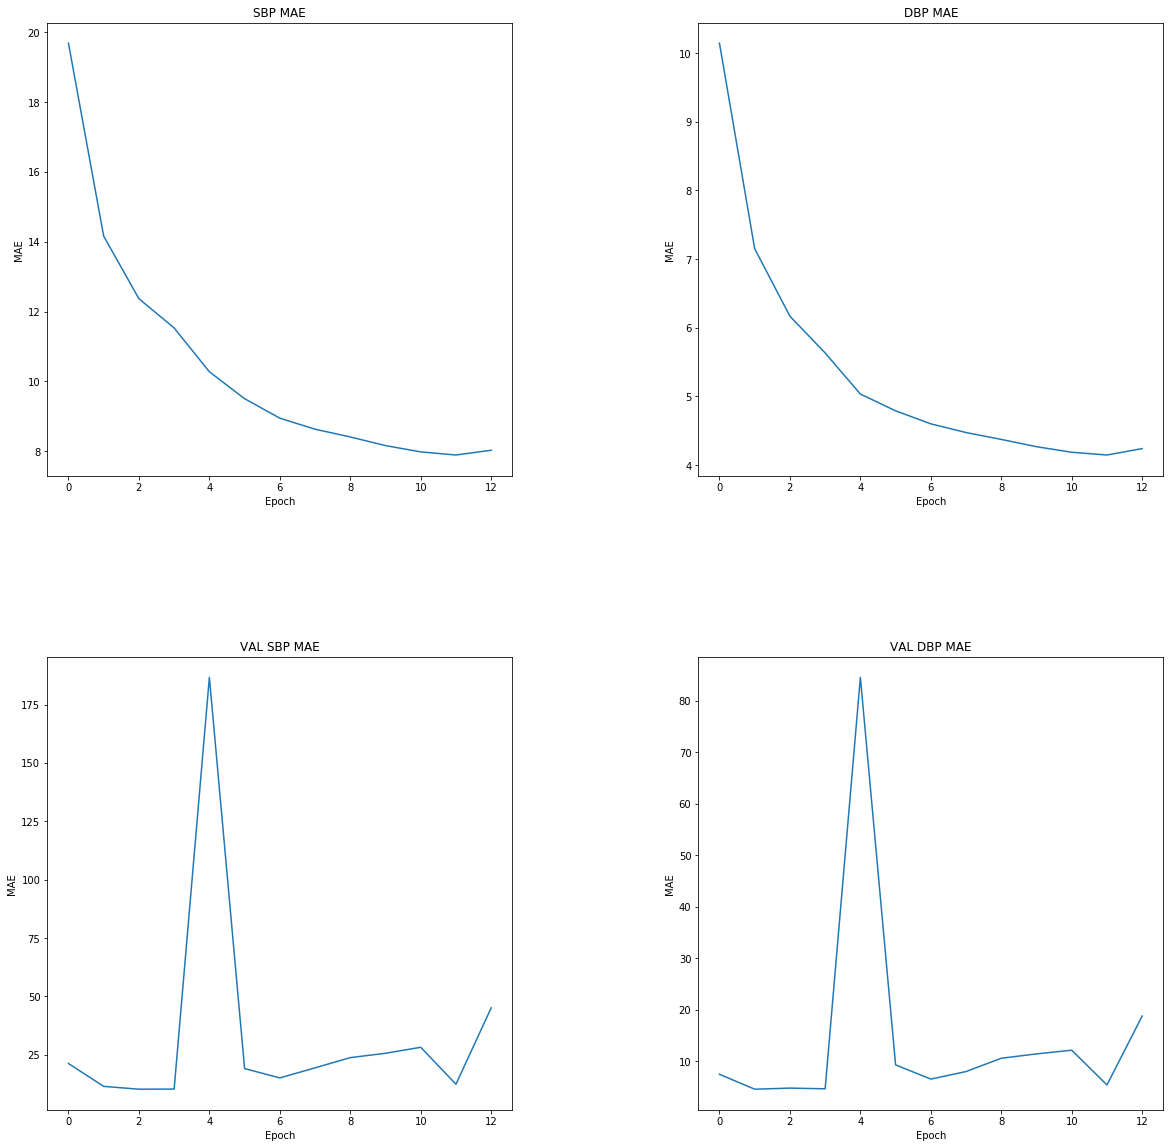
\includegraphics[width=10cm,height=10cm,keepaspectratio]{Results/alexnet.png}
    \caption{MAE of SBP and DBP for AlexNet architecture}
    \label{alexnetResults}
\end{figure}

\subsection{Performance of ResNet architecture}

\begin{figure}[H]
    \centering
    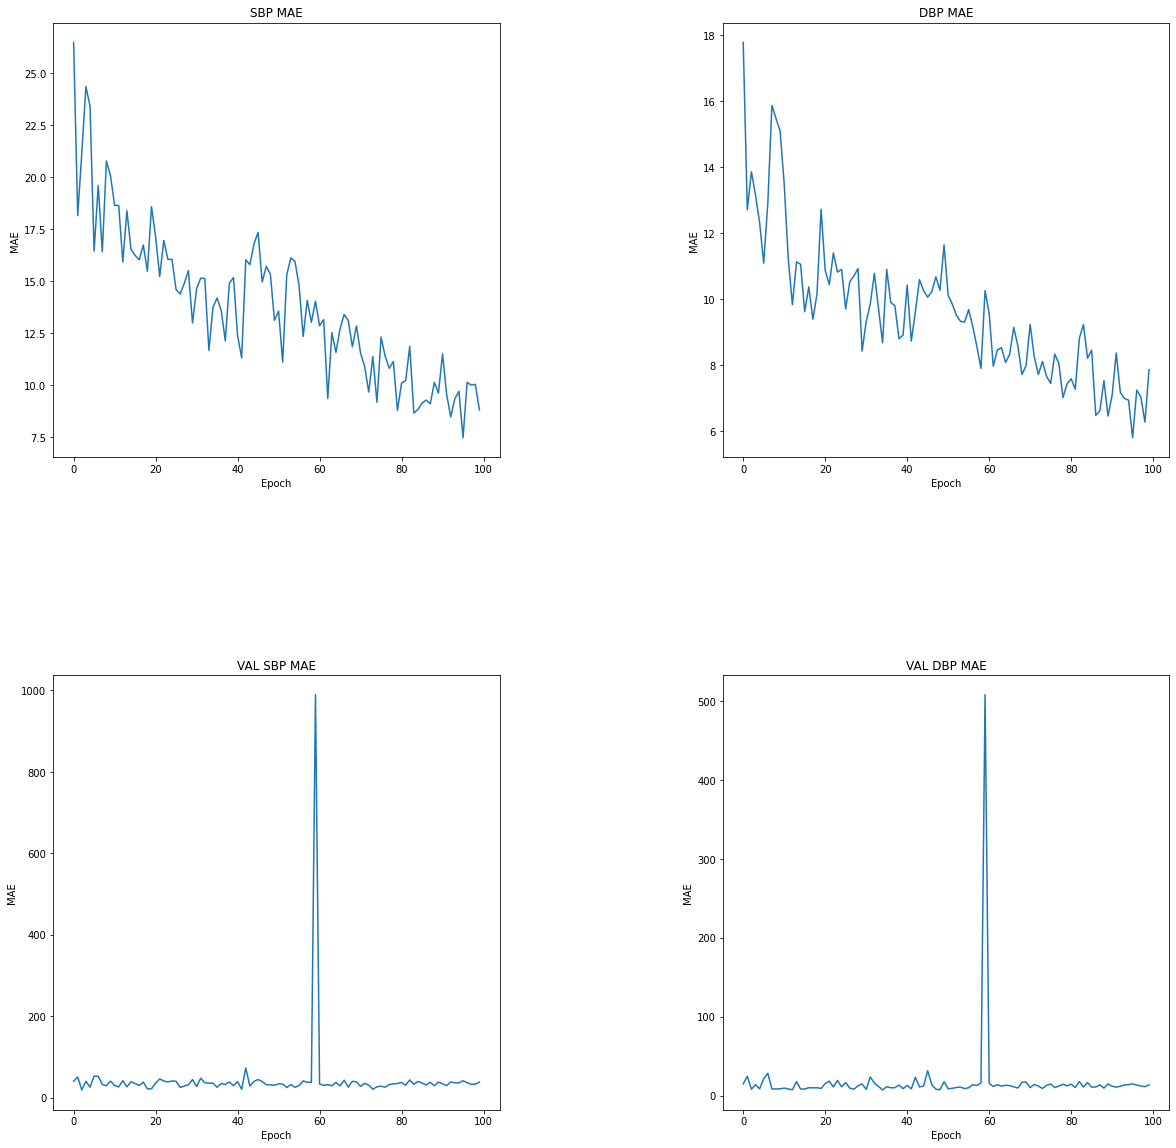
\includegraphics[width=15cm,height=15cm,keepaspectratio]{Results/resnet.png}
    \caption{MAE of SBP and DBP for ResNet architecture}
    \label{resnetResults}
\end{figure}